\documentclass[11pt]{report}

% Paquetes y configuraciones adicionales
\usepackage[spanish]{babel} % Cargar el paquete babel con la opción en español
\usepackage{graphicx}
\usepackage[export]{adjustbox}
\usepackage{caption}
\usepackage{float}
\usepackage{titlesec}
\usepackage{geometry}
\usepackage[hidelinks]{hyperref}
\usepackage{parskip}
\usepackage{hyperref}
\usepackage{nameref}
\usepackage{listings}
\usepackage{wrapfig}

% Configura los márgenes
\geometry{
    left=2cm,   % Ajusta este valor al margen izquierdo deseado
    right=2cm,  % Ajusta este valor al margen derecho deseado
    top=2cm,
    bottom=2cm,
}

% Redefinir el formato del capítulo
\titleformat{\chapter}[block]
  {\normalfont\huge\bfseries}{\chaptertitlename\ \thechapter}{1em}{\Huge}

% Ajustar el espaciado antes y después del título del capítulo
\titlespacing*{\chapter}{0pt}{0pt}{20pt}

% Configuración de los títulos de las secciones
\titlespacing{\section}{0pt}{\parskip}{\parskip}
\titlespacing{\subsection}{0pt}{\parskip}{\parskip}
\titlespacing{\subsubsection}{0pt}{\parskip}{\parskip}

\begin{document}

% Portada del informe

\title{Linked Data}
\author{Samuel Martín Morales  \texttt{alu0101359526@ull.edu.es}}
\date{\today}

\maketitle

% Índice
\tableofcontents

\chapter{Visualización de tres categorías de scripts}

Para comenzar con la quinta práctica de la asignatura de \emph{\textbf{Tecnologías de la Información en las Organizaciones}} se solicita el empleo de scripts de R que permiten la visualización de los distintos datos que posee el dataset, siendo que, para este caso se trata del dataset número 23. Además, cabe destacar que los scripts de R usados no solo se han empleado para la visualización de los datos, sino que también se han empleado para la implementación de un algoritmo de \emph{Random-Forest}, el cual permite realizar un análisis predictivo.

\section{Script de correlación}

En primer lugar se ha empleado un script de R que permite la visualización de la correlación entre los distintos atributos del dataset. El scrip`t' seleccionado se trata del fichero denominado como \emph{Corr\_4.r}. Dicho script de manera inicial, se encontraba de la siguiente manera:

\begin{lstlisting}[language=R, breaklines=true, basicstyle=\small\ttfamily]
library(corrplot)
mtcars.cor <- cor(dataset, method = "spearman")
round(mtcars.cor,2)
col <- colorRampPalette(c("#BB4444", "#EE9988", "#FFFFFF",
                          "#77AADD","#4477AA"))		 
corrplot(mtcars.cor, method = "pie", shade.col = NA, tl.col = "black",
          tl.srt = 45, col = col(200), addCoef.col = "black", addcolorlabel = "no",
          order = "AOE", type = "upper", diag = F, addshade = "all")	
\end{lstlisting}

Teniendo en cuenta el script anterior, se realizan una serie de modificaciones para la visualización de la correlación entre los distintos atributos del dataset. Estas, se basan de manera principal en la personalización de los colores de la representación y del método de graficación usado. En este caso, se hace uso del method \emph{circle} en vez de hacer uso del método \emph{pie}.

Todo esto mencionado se puede ver a continuación:

\begin{lstlisting}[language=R, breaklines=true, basicstyle=\small\ttfamily]
  library(corrplot)
  mtcars.cor <- cor(dataset, method = "spearman")
  round(mtcars.cor,2)
  col <- colorRampPalette(c("#4575b4", "#91bfdb", "#fee08b", "#d73027"))				 
  corrplot(mtcars.cor, method = "circle", shade.col = NA, tl.col = "black",
           tl.srt = 45, col = col(200), addCoef.col = "black", addcolorlabel = "no",
           order = "AOE", type = "upper", diag = F, addshade = "all", main = "Matriz de correlación", xlab = "Variables", ylab = "Variables")	
\end{lstlisting}

Finalmente, la visualización obtenida es la siguiente:

\begin{figure}[H]
	\centering
	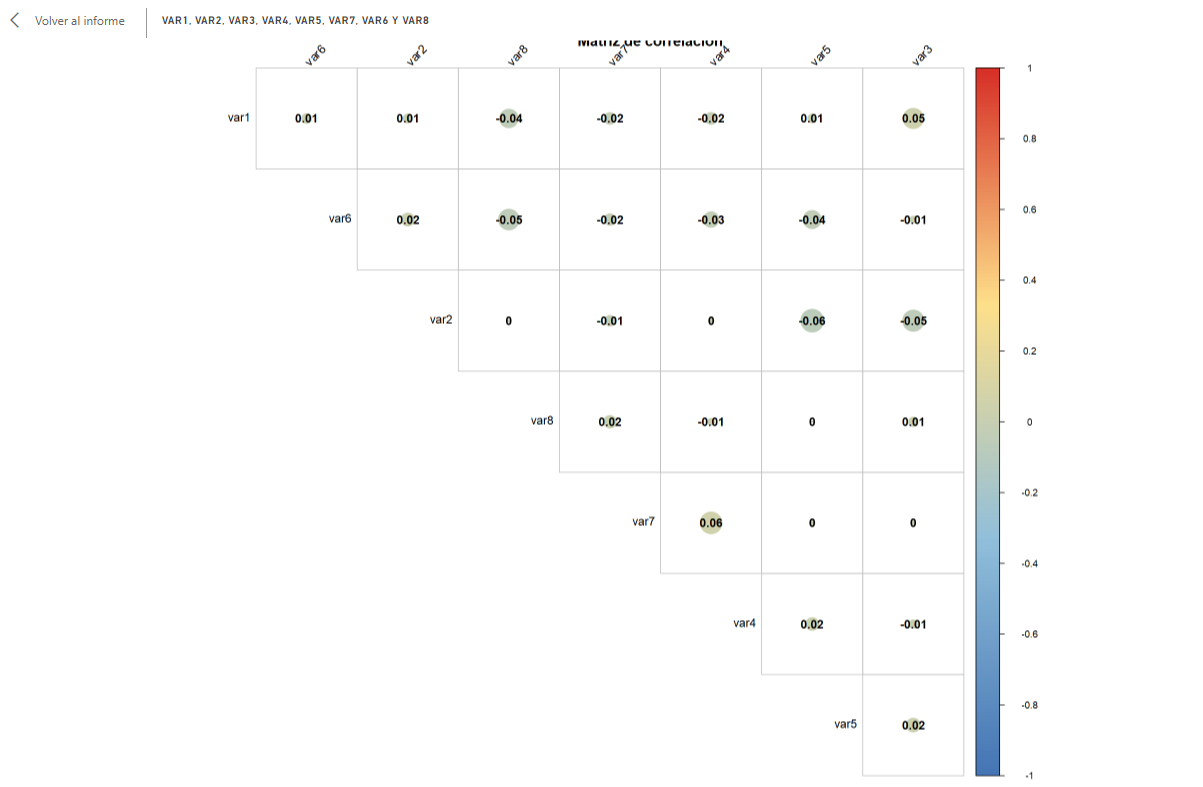
\includegraphics[width=0.9\textwidth]{./img/Correlation-Image.png}
	\caption{Visualización de la correlación entre los distintos atributos del dataset}
	\label{fig:correlation}
\end{figure}

\section{Script de Densidad}

Para continuar con la visualización de los datos, se ha empleado un script de R que permite la visualización de la densidad de los atributos 1 y 2. El script seleccionado se trata del fichero denominado como \emph{Dens\_1.r}. Dicho script de manera inicial, se encontraba de la siguiente manera:

\begin{lstlisting}[language=R, breaklines=true, basicstyle=\small\ttfamily]
library(ggplot2)
library(hrbrthemes)
# Chart
p <- ggplot(dataset, aes(x=x) ) +
  # Top
  geom_density( aes(x = var1, y = ..density..), fill="#69b3a2" ) +
  geom_label( aes(x=4.5, y=0.25, label="Variable 1"), color="#69b3a2") +
  # Bottom
  geom_density( aes(x = var2, y = -..density..), fill= "#404080") +
  geom_label( aes(x=4.5, y=-0.25, label="Variable 2"), color="#404080") +
  theme_ipsum() +
  xlab("value of x")
p
\end{lstlisting}

Para la modificación o la personalización de la representación que genera el comentado script, se hace uso del cambio de la paleta de colores usados mediante una librería denominada como \emph{viridis}. Además, se ha modificado el título y los ejes de la representación. Todo esto mencionado se puede ver a continuación:

\begin{lstlisting}[language=R, breaklines=true, basicstyle=\small\ttfamily]
library(ggplot2)
library(hrbrthemes)
library(viridis)

# Se realiza la creación de la paleta de colores que se va a usar para el top y para el bottom
color_palette_top <- viridis(2)[1]
color_palette_bottom <- viridis(2)[2]

# Chart
p <- ggplot(dataset, aes(x = x)) +
  # Top
  geom_density(aes(x = var1, y = ..density..), fill = color_palette_top, alpha = 0.7) +
  geom_label(aes(x = 4.5, y = 0.25, label = "Variable 1"), color = color_palette_top) +
  # Bottom
  geom_density(aes(x = var2, y = -..density..), fill = color_palette_bottom, alpha = 0.7) +
  geom_label(aes(x = 4.5, y = -0.25, label = "Variable 2"), color = color_palette_bottom) +
  theme_ipsum() +
  xlab("Value of x") +
  ylab("Density") +
  labs(title = "Distribuciones de Variable 1 y 2", subtitle = "Realizado por Samuel Martín Morales") + 
  theme(
    plot.title = element_text(hjust = 0.5),  # Se establecen las características de los textos
    plot.subtitle = element_text(hjust = 0.5),  
    legend.position = "bottom",  
    legend.direction = "horizontal",  
    legend.box = "horizontal"  
  )

p
\end{lstlisting}

Finalmente, la visualización obtenida es la siguiente:

\begin{figure}[H]
  \centering
  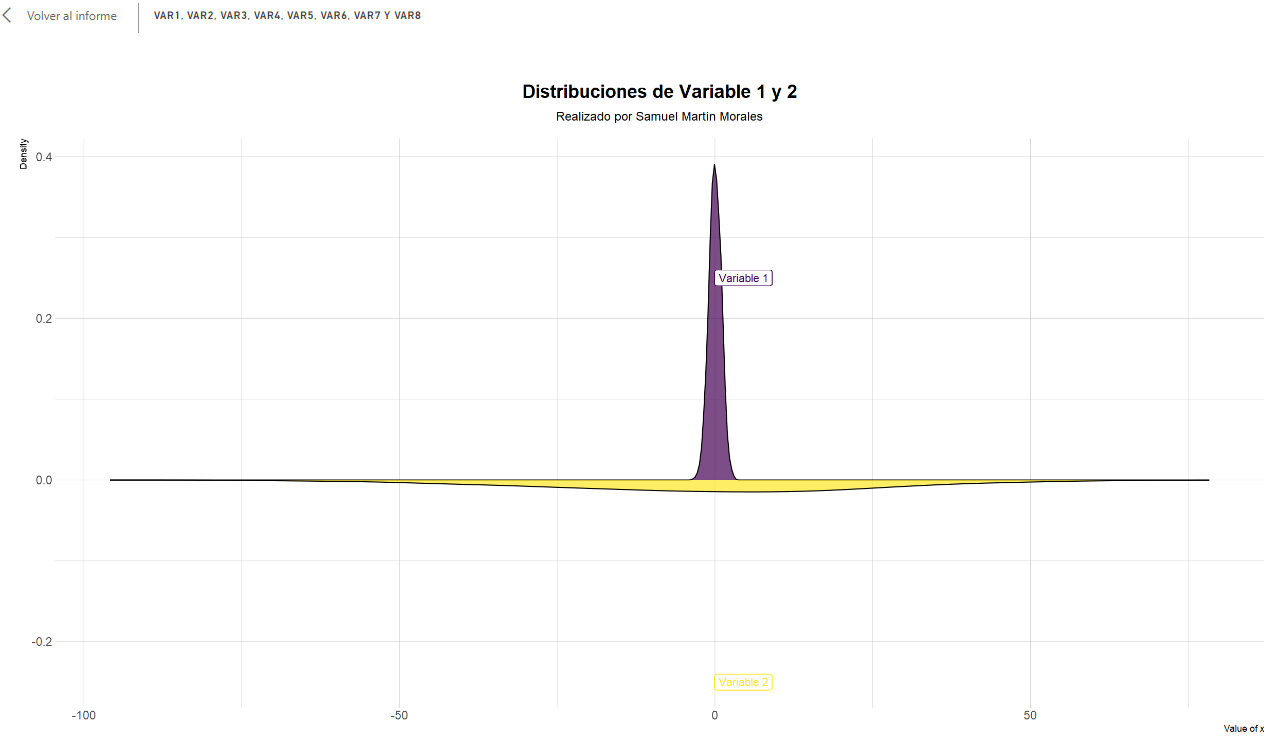
\includegraphics[width=0.9\textwidth]{./img/Density-Image.png}
  \caption{Visualización de la densidad de los atributos 1 y 2}
  \label{fig:density}
\end{figure}

\section{Script de clustering}

Para finalizar, se ha empleado un script de R que permite la visualización de los datos mediante el uso de un algoritmo de clustering con un tamaño de \emph{K }de 3 . El dataset seleccionado se trata del fichero denominado como \emph{Kmean\_2.r}. Dicho script de manera inicial, se encontraba de la siguiente manera:

\begin{lstlisting}[language=R, breaklines=true, basicstyle=\small\ttfamily]
library(ggpubr)
library(factoextra)
# Compute k-means with k = 3
set.seed(123)
res.km <- kmeans(scale(dataset), 3, nstart = 25)

fviz_cluster(res.km, data = dataset,
              palette = c("#2E9FDF", "#00AFBB", "#E7B800"), 
              geom = "point",
              ellipse.type = "convex", 
              ggtheme = theme_bw()
              )
\end{lstlisting}

Para la personalización de la representación que genera el script, se hace uso de nuevo de la librería \emph{viridis} para la modificación de la paleta de colores usados. Además, se ha modificado el título y los ejes de la representación. Todo esto mencionado se puede ver a continuación:

\begin{lstlisting}[language=R, breaklines=true, basicstyle=\small\ttfamily]
library(ggpubr)
library(factoextra)
library(viridis)

# Cambiar la paleta de colores
my_palette <- viridis(3)

# Calcular k-means con k = 3
set.seed(123)
res.km <- kmeans(scale(dataset), 3, nstart = 25)

# Personalizar el gráfico
p <- fviz_cluster(
  res.km, 
  data = dataset,
  palette = my_palette,
  geom = "point",
  ellipse.type = "convex",
  ggtheme = theme_minimal(),  # En este punto se realiza el cambio de tema
  main = "Análisis de Clústeres",
  xlab = "Variable 1",  
  ylab = "Variable 2"   
)

# Implementación de algunos tipos de configuraciones de los distintos textos
p + theme(
  legend.position = "bottom",  
  legend.title = element_blank(), 
  plot.title = element_text(size = 16, face = "bold"),  
  plot.subtitle = element_text(size = 14, face = "italic"),  
  axis.title = element_text(size = 12, face = "bold")  
)
\end{lstlisting}

Finalmente, la visualización obtenida es la siguiente:

\begin{figure}[H]
  \centering
  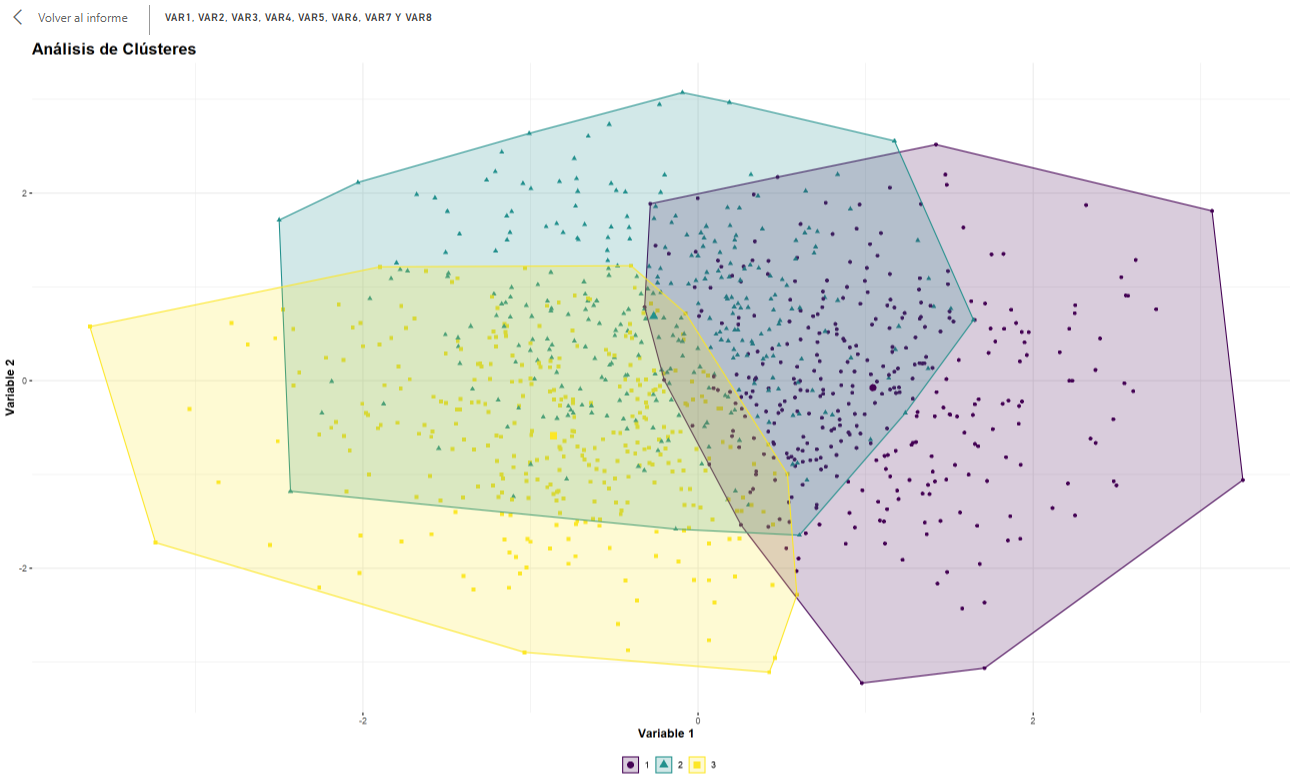
\includegraphics[width=0.9\textwidth]{./img/Clusters-Image.png}
  \caption{Visualización de los datos mediante el uso de un algoritmo de clustering con un tamaño de \emph{K } = 3}
  \label{fig:clustering}
\end{figure}

\chapter{Visualización de dos scripts personalizados}

Dentro del segundo ejercicio, se solicita la implementación de dos visualizaciones personalizadas, que, hagan uso de alguna de las decenas librerías de R, de tal manera que permitan la visualización de los datos de nuevas formas y de otras maneras distintas a las que se han empleado en el ejercicio anterior.

\section{Primera representación personalizada}

La primera de las visualizaciones personalizadas se basa en la representación de los datos mediante un gráfico que muestre las relaciones que existen entre pares de variables, de tal manera que se puedan identificar patrones y correlaciones entre las distintas variables. De forma más concreta, se trata de un gráfico de pares sobre las variables o atributos del dataset denominadas como \emph{var1} , \emph{var2}, \emph{var3} y \emph{var4}.

Todo esto comentado anteriormente, queda representado en el siguiente script:

\begin{lstlisting}[language=R, breaklines=true, basicstyle=\small\ttfamily]
library(ggplot2)
library(GGally)

# Crear un gráfico de pares
ggpairs(dataset, columns = c("var1", "var2", "var3", "var4"), 
        title = "Gráfico de Pares")
\end{lstlisting}

Finalmente, la visualización obtenida es la siguiente:

\begin{figure}[H]
  \centering
  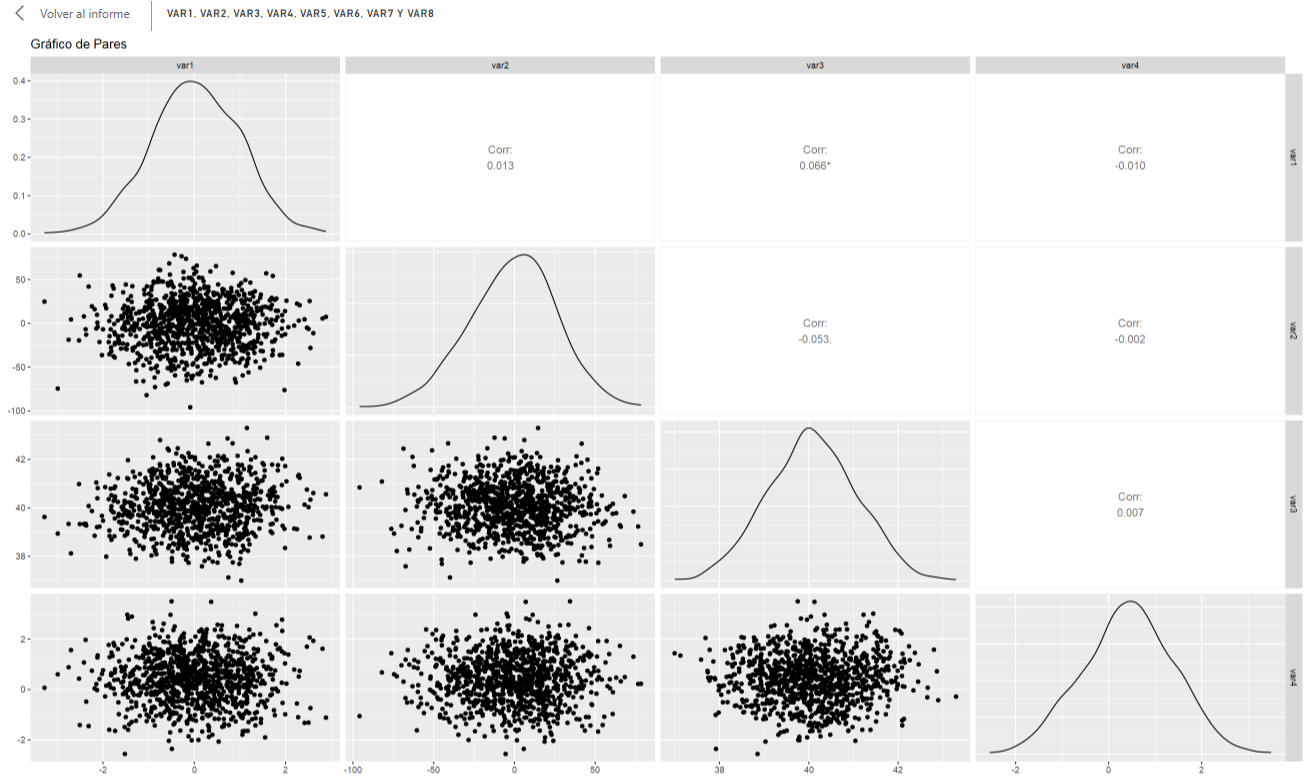
\includegraphics[width=0.9\textwidth]{./img/Pair-Graph-Image.png}
  \caption{Visualización de los datos mediante un gráfico de pares}
  \label{fig:pair}
\end{figure}

\section{Segunda representación personalizada}

La segunda y última de las visualizaciones personalizadas se basa en la representación de los datos mediante un mapa de calor a partir del cálculo de la correlación entre los atributos del dataset. Dicha visualización hace uso del siguiente script:

\begin{lstlisting}[language=R, breaklines=true, basicstyle=\small\ttfamily]
library(pheatmap)
library(RColorBrewer)

mtcars.cor <- cor(dataset, method = "spearman")
round(mtcars.cor,2)
pheatmap(mtcars.cor, color = colorRampPalette(brewer.pal(10, "Blues"))(200), 
          main = "Mapa de Calor de la Matriz de Correlación")
\end{lstlisting}

Finalmente, la visualización obtenida es la siguiente:

\begin{figure}[H]
  \centering
  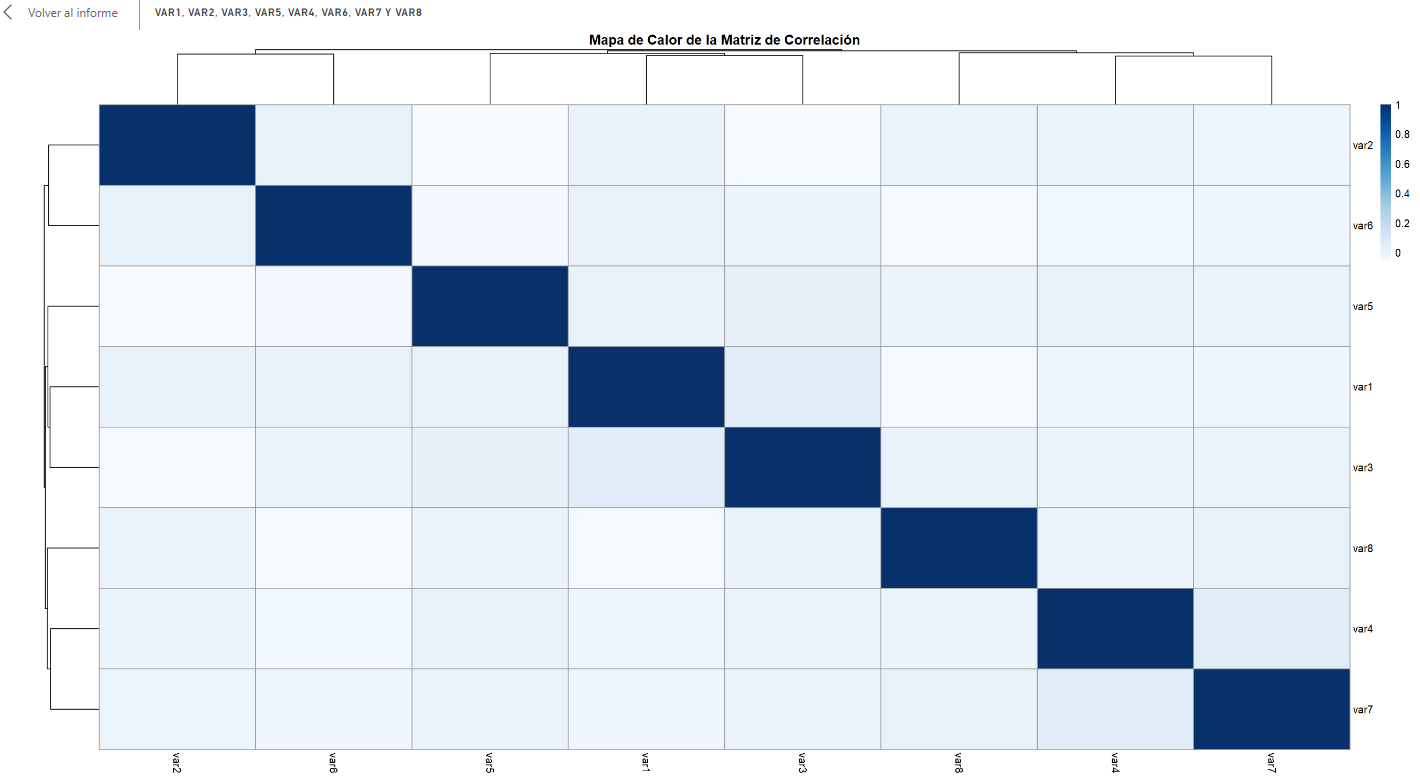
\includegraphics[width=0.9\textwidth]{./img/Heat-Map-Correlation-Image.png}
  \caption{Visualización de los datos mediante un mapa de calor a partir del cálculo de la correlación entre los atributos del dataset}
  \label{fig:heatmap}
\end{figure}

\chapter{Implementación del algoritmo \emph{Random-Forest}}

Para la finalización de la práctica, se solicita la implementación de un algoritmo de \emph{Random-Forest} que permita realizar un análisis predictivo sobre los datos del dataset usado dentro de la práctica tutorizada realiza de manera previa a la implementación de esta práctica. Dicho dataset se trata de un dataset que presenta la distintas características que presentan diferentes tipos de hormigón.

Para la realización de una análisis predictivo se hace uso del script que se puede observar a continuación. También cabe destacar que una vez se realiza el entrenamiento del análisis predictivo, se realiza la visualización de los resultados obtenidos mediante la librería \emph{ggplot2}. Por tanto, se tiene el siguiente script utilizado para ello:

\begin{lstlisting}[language=R, breaklines=true, basicstyle=\small\ttfamily]
  library(randomForest)
  library(ggplot2)
  
  concrete_data <- dataset
  
  # Establecimiento de la semilla
  set.seed(123)
  
  # Creación de distintos conjuntos de datos para entrenamiento y prueba
  train_index <- sample(1:nrow(concrete_data), 0.7 * nrow(concrete_data))
  train_data <- concrete_data[train_index, ]
  test_data <- concrete_data[-train_index, ]
  
  # Entrenamiento del modelo RandomForest
  modelo_rf <- randomForest(strength ~ ., data = train_data)
  
  predicciones <- predict(modelo_rf, newdata = test_data)
  
  ggplot(data = data.frame(Real = test_data$strength, Predicho = predicciones)) +
    geom_point(aes(x = Real, y = Predicho)) +
    geom_abline(slope = 1, intercept = 0, color = "red", linetype = "dashed") +
    labs(title = "Relación entre Valores Reales y Predichos",
         x = "Valor Real",
         y = "Valor Predicho")
  
  
  # Visualización de la estructura de los primeros dos árboles (se puede ajustar según se necesite)
  # tree1 <- getTree(modelo_rf, k = 1)
  
  # Visualización de la estructura del primer árbol
  # print(tree1)
\end{lstlisting}

Finalmente, la visualización obtenida sobre el análisis predictivo realizado es la siguiente:

\begin{figure}[H]
  \centering
  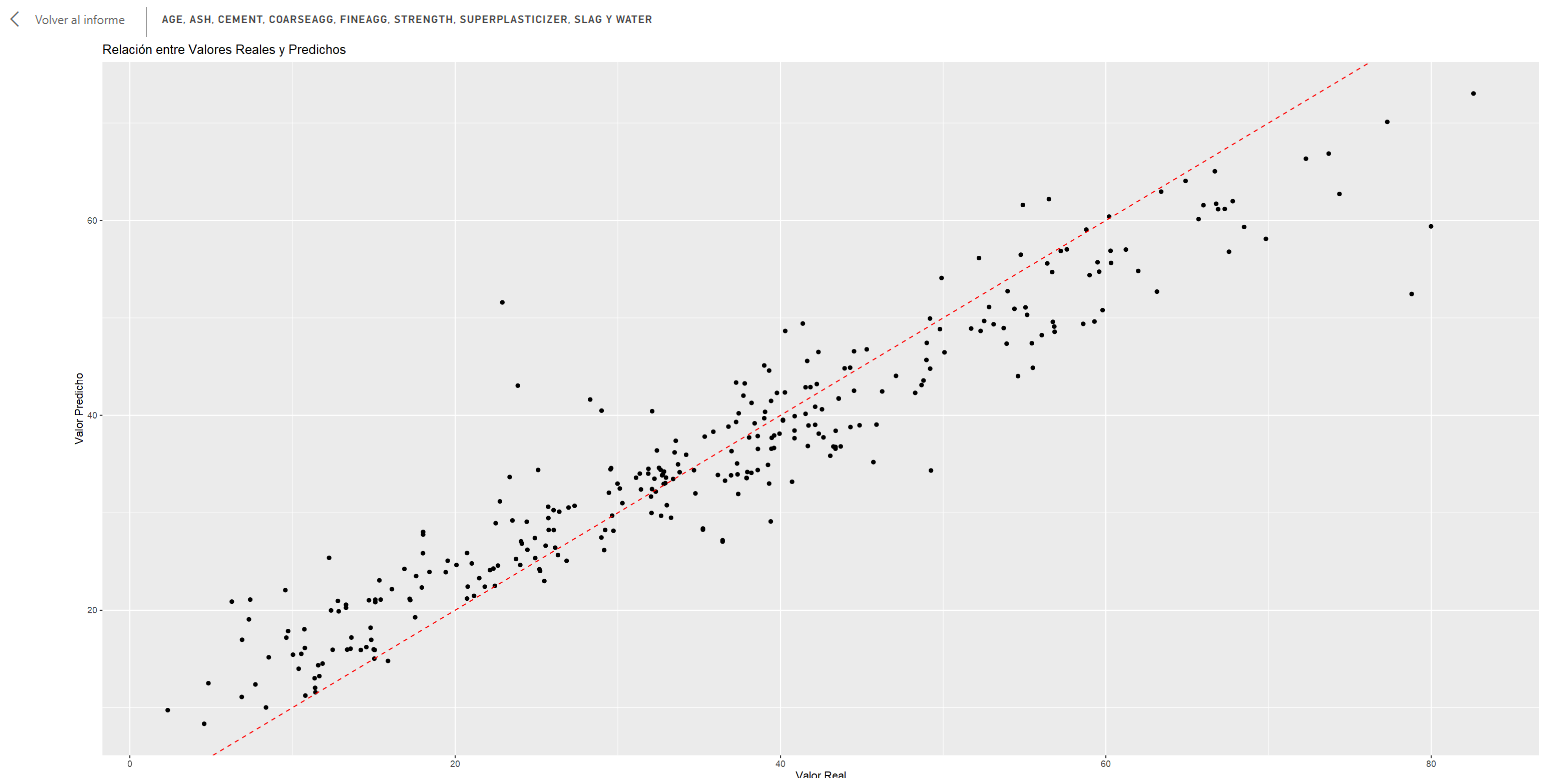
\includegraphics[width=0.9\textwidth]{./img/Random-Forest-Image.png}
  \caption{Visualización de los datos mediante una nube de puntos que muestra la relación entre los valores reales y los valores predichos}
  \label{fig:randomForest}
\end{figure}

Para concluir, se tienen los distintos scripts de R usados para la realización de la práctica en el repositorio de GitHub \cite{1} y el fichero de PowerBI en el repositorio de Google Drive \cite{2}.

\begin{thebibliography}{99}
  \bibitem{1} Samuel. (2023). Visualization-Tecnology. GitHub. \url{https://github.com/Samuelmm15/Visualization-Tecnology}
  \bibitem{2} Samuel. (2023). PowerBI-File. Google Drive. \url{https://github.com/Samuelmm15/Visualization-Tecnology}
\end{thebibliography}

\end{document}